\documentclass[twocolumn]{class}


\addbibresource{References.bib}

% add path to images
\graphicspath{ {./images/} }

\title{Heart Disease Prediction from heart beat audio signals using Machine Learning and Network Analysis}
\shorttitle{Heart Disease Prediction}

\github{https://github.com/DavideLigari01/advanced-biomedical-project}

\author{Ligari D. • Alberti A.  }

\affil[1]{Department of Computer Engineering, Data Science, University of Pavia, Italy \newline\centering Course of Advanced Biomedical Machine Learning}

\keywords{---TO BE DEFINED---}
\abstract{  
   ---TO BE DEFINED---
}
\firstauthor{Alberti Ligari}
\publicationdate{\today}


\begin{document}

\maketitle
\pagestyle{FirstPage}

\tableofcontents
% \nocite{dizdar_dns_2021}

% ------------------- START OF SECTIONS -------------------


% ------------------- Introduction -------------------

% Introduction to the medical problem and how it is currently addressed (some bibliography)
\section{Introduction}
\pagestyle{OtherPage}

% ------------------- Diseases -------------------


\section{Dataset}
\section{Dataset Description}

The dataset for this project was obtained from a Kaggle repository titled \textit{Dangerous Heartbeat Dataset (DHD)} \cite{Dangerous-Heartbeat-Dataset-DHD}, 
which in turn sources its data from the PASCAL Classifying Heart Sounds Challenge 2011 (CHSC2011) \cite{pascal-chsc-2011}. 
This dataset comprises audio recordings of heartbeats, categorized into different types of heart sounds.
Specifically, the dataset consists of 5 types of recordings: Normal Heart Sounds, Murmur Sounds, Extra Heart Sounds, Extrasystole Sounds, and Artifacts.
Data has been gathered from the general public via the iStethoscope Pro iPhone app and from a clinic trial in hospitals using the digital stethoscope DigiScope.


% ------------------- Dataset -------------------

% Description of the dataset and its features (some plots and one hot encoding)
\section{Heart Sound Categories}
Heart sounds can be categorized into different classes based on their acoustic characteristics and clinical significance.
Accurate classification of these sounds is essential for diagnosing and treating a variety of cardiac conditions.
The primary categories include Normal heart sounds, Murmurs, Extra Heart Sounds, Artifacts, and Extra Systoles.
Understanding the distinct features and clinical implications of each class is a crucial step before building a
machine learning model to classify heartbeats.
This phase is particularly important for the identification of patterns that are characteristic of specific classes,
which in turn guides the selection of features to extract from the audio.
This knowledge aids in identifying specific patterns and anomalies within the heart sounds,
leading to more precise and reliable model predictions.
\subsection{Normal}
The Normal category includes recordings of typical, healthy heart sounds. These sounds exhibit the characteristic ``lub-dub, lub-dub'' pattern,
where ``lub'' (S1) represents the closing of the atrioventricular valves and ``dub'' (S2) signifies the closing of the semilunar valves.
In a normal heart, the time interval between ``lub'' and ``dub'' is shorter than the interval from ``dub'' to the next ``lub,''
especially when the heart rate is below 140 beats per minute. Most normal heart rates at rest fall between 60 and 100 beats per minute,
though rates can vary from 40 to 140 beats per minute based on factors such as age and activity level.
Recordings may include background noises like traffic or radio sounds and may capture incidental noises such as breathing or microphone
contact with clothing or skin. It contains both clean and noisy normal recordings,
the latter featuring significant background noise or distortion, which simulates real-world conditions.\\
Figure \ref{fig:normal_heart_beat_audio} shows a sample of a normal heart beat audio.
The characteristic ``lub-dub, lub-dub'' pattern can be observed, where the peaks represent the ``lub'' (S1) and ``dub'' (S2) sounds of a healthy heart.

\begin{figure}[H]
    \centering
    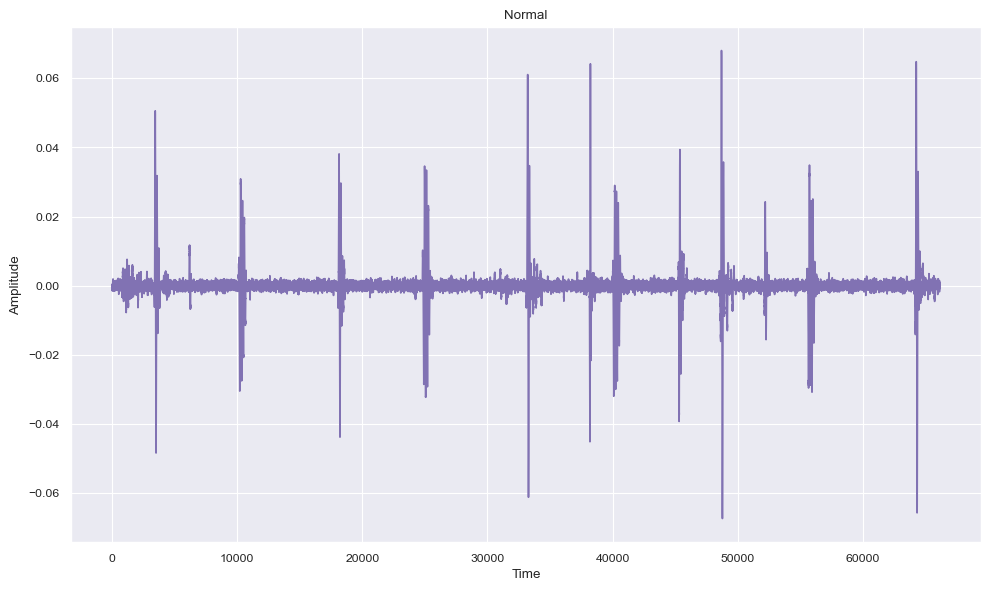
\includegraphics[width=.8\columnwidth]{../images/normal_heart_beat_audio.png}
    \caption{Sample of normal heart beat audio.}
    \label{fig:normal_heart_beat_audio}
\end{figure}
\noindent




\subsection{Murmur}
Heart murmurs are abnormal sounds during the heartbeat cycle, such as a ``whooshing, roaring, rumbling, or turbulent fluid'' noise, heard between
the ``lub'' and ``dub'' (systolic murmur) or between ``dub'' and ``lub'' (diastolic murmur).
These murmurs are typically indicative of turbulent blood flow in the heart and can signal various heart conditions, some of which may be serious.
It is crucial to distinguish murmurs from the normal ``lub-dub'' sounds since they occur between the primary heart sounds and not concurrently with them.
It also includes noisy murmur data, which mimics real-world recording scenarios by incorporating significant background noise and distortions.\\
Figure \ref{fig:murmur_heart_beat_audio} shows a sample of a murmur heart beat audio.
The presence of additional sounds between the ``lub'' and ``dub'' peaks can be observed, indicating the characteristic
``whooshing, roaring, rumbling, or turbulent fluid'' noise typical of heart murmurs.

\begin{figure}[H]
    \centering
    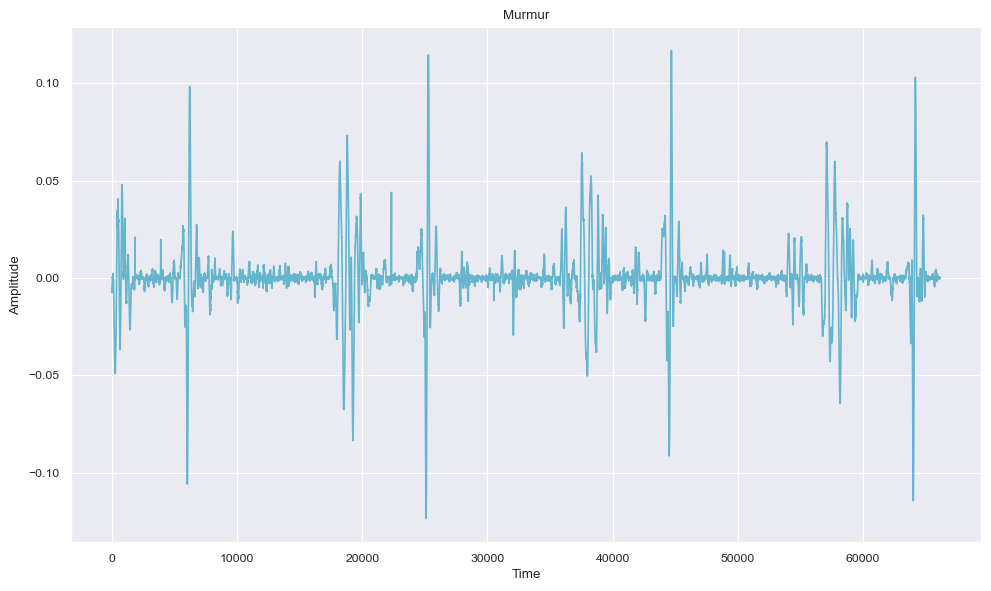
\includegraphics[width=.8\columnwidth]{../images/murmur_heart_beat_audio.png}
    \caption{Sample of murmur heart beat audio.}
    \label{fig:murmur_heart_beat_audio}
\end{figure}
\noindent


\subsection{Extra Heart Sound}
Extra heart sounds are characterized by an additional sound in the cardiac cycle, producing patterns such as ``lub-lub dub'' or ``lub dub-dub''.
These sounds can arise from physiological or pathological conditions. For example, a third heart sound (S3) may indicate heart failure or volume overload,
while a fourth heart sound (S4) can be associated with a stiff or hypertrophic ventricle.
Detecting these extra sounds is important for identifying potential heart diseases early, allowing for timely intervention and management.
Figure \ref{fig:extrahls_heart_beat_audio} shows a sample of an extra heart sound audio.
The presence of additional peaks within the normal ``lub-dub'' pattern indicates extra heart sounds, which can be
critical for diagnosing various heart conditions.

\begin{figure}[H]
    \centering
    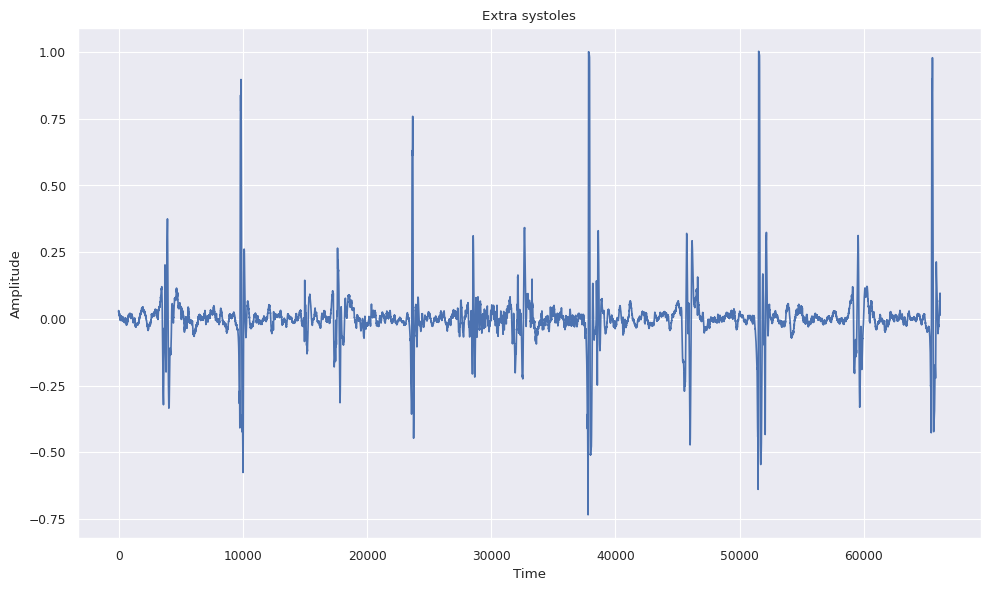
\includegraphics[width=.8\columnwidth]{../images/extrastoles_heart_beat_audio.png}
    \caption{Sample of extra heart sound audio.}
    \label{fig:extrahls_heart_beat_audio}
\end{figure}
\noindent

\subsection{Artifact}
The Artifact category consists of recordings with non-cardiac sounds, including feedback squeals, echoes, speech, music, and various types of noise.
These recordings generally lack discernible heart sounds and do not exhibit the temporal periodicity typical of heartbeats at frequencies below 195 Hz.
Accurately identifying artifacts is essential to avoid misinterpreting non-cardiac sounds as pathological heart sounds,
ensuring that data collection efforts focus on genuine heart sounds.
Figure \ref{fig:artifact_heart_beat_audio} shows a sample of an artifact heart beat audio, there can be observed that there is not a clear pattern in the audio.

\begin{figure}[H]
    \centering
    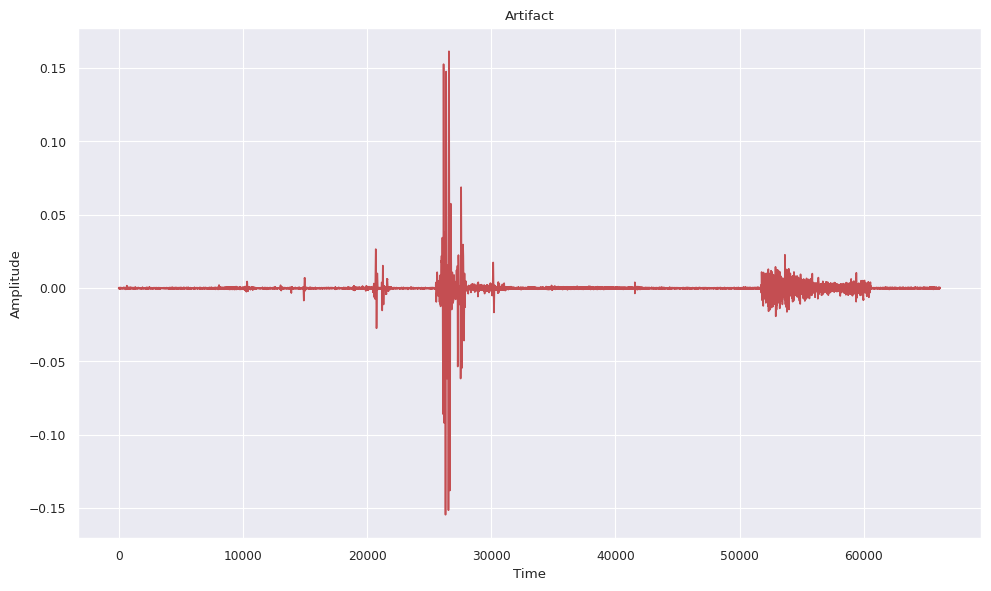
\includegraphics[width=.8\columnwidth]{../images/artifact_heart_beat_audio.png}
    \caption{Sample of artifact heart beat audio }\label{fig:artifact_heart_beat_audio}
\end{figure}
\noindent
\subsection{Extra systoles}
Extra systoles refers to extra or skipped heartbeats, resulting in irregular patterns such as ``lub-lub dub'' or ``lub dub-dub''.
Unlike the regular extra heart sounds, extra systoles are sporadic and do not follow a consistent rhythm.
These premature beats can occur in healthy individuals, particularly children, but they may also be associated with various heart diseases.
Identifying extra systoles is crucial as they can be early indicators of cardiac conditions that might require medical attention
if they occur frequently or in certain patterns.\\
In the audio signal depicted in Figure \ref{fig:extrastoles_heart_beat_audio}, irregularities within the normal “lub-dub” pattern are evident.
These irregularities manifest as additional peaks or skipped beats, indicating extra systoles.
\begin{figure}[H]
    \centering
    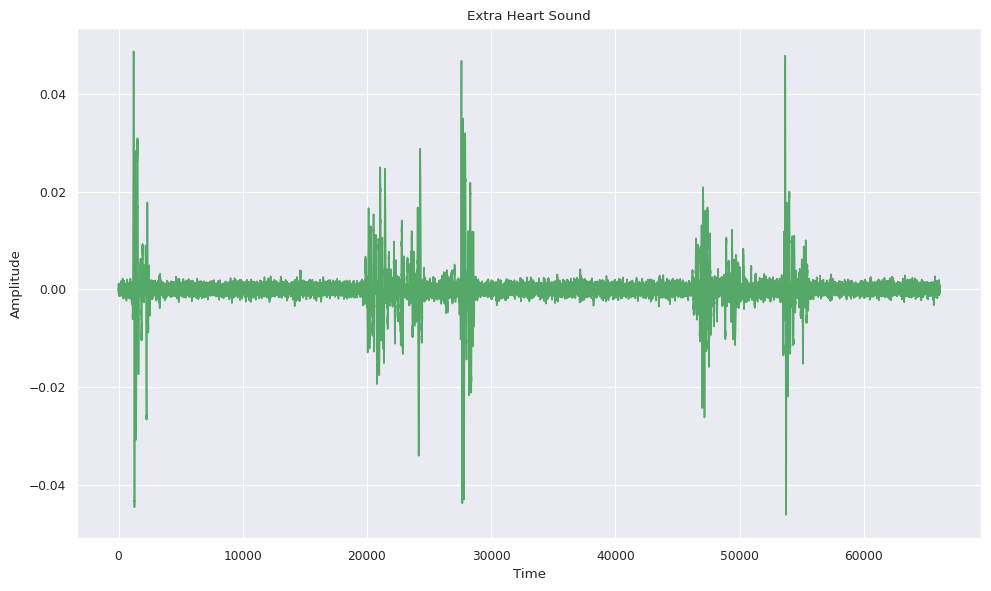
\includegraphics[width=.8\columnwidth]{../images/extrahls_heart_beat_audio.png}
    \caption{Sample of extra systoles heart beat audio }\label{fig:extrastoles_heart_beat_audio}
\end{figure}
\noindent
\subsection{Comparison of Heart Sounds}
In Figure \ref{fig:comparison_heart_beat_audio}, a comparison of the different classes of heart sounds can be observed.\\
As we can see, the “Artifact” signal appears erratic with no consistent pattern, likely representing noise or interference rather than true heart sounds.\\
The “Murmurs” signal shows irregular fluctuations in amplitude, which could indicate turbulent blood flow typically associated with murmurs. \\
The signal for “Extra Heart Beat Sound” has occasional spikes in amplitude that stand out from the baseline.\\
The “Normal” signal appears more uniform and regular compared to the others, reflecting the expected rhythm of a healthy heartbeat.
FInally, the signal for “Extra Systoles” shows extra spikes at irregular intervals,
indicating unexpected contractions of the heart muscle (systoles) occurring outside the normal rhythm.

\begin{figure}[H]
    \centering
    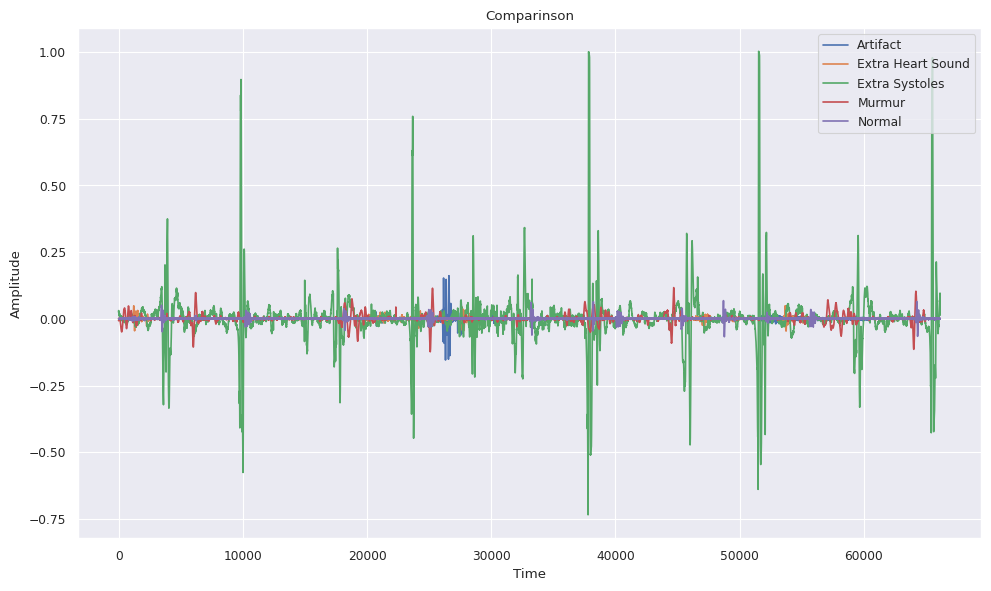
\includegraphics[width=.8\columnwidth]{../images/comparison_heart_beat_audio.png}
    \caption{Comparison of the different classes of heart sounds.}
    \label{fig:comparison_heart_beat_audio}
\end{figure}
\noindent



% ------------------- Goals -------------------

% Description of the goals of the project:
\section{Goals}
% - ML model to predict the disease
% - Network analysis to find the most important symptoms to reduce complexity, and enhance the available features


% -------------------Feature extraction -------------------

\section{Feature Extraction}


\subsection{MFCC}
\subsection{Chroma}
\subsection{RMS}
\subsection{ZCR}
\subsection{CQT}
\subsection{Spectral Centroid}
\subsection{Spectral Bandwidth}
\subsection{Spectral Roll-off}

\subsection{Sample rate and interval selection}

\subsection{Results}





% ------------------- Feature Selection -------------------
\section{Feature Selection}
This phase serves a dual purpose. Firstly, since each type of feature (MFCC, Chroma, CQT, etc.) can consist of a varying number of individual features,
it is important to determine the optimal number of features for each type to maximize the model's performance.
Secondly, this phase aims to identify which specific features are the most relevant and influential for the classification task.
By doing so, we can enhance the model's efficiency and accuracy by focusing on the features that contribute the most to the classification process.

\subsection{Optimal number of features for each type of feature}
Considering that each type of feature can consist of a variable number of individual features,
it is necessary to determine the optimal number of features for each type to maximize the model's performance.
To achieve this, a `One Model per Feature' approach was employed. This involved training a separate model for each type of feature,
varying the number of features used. A set of 12, 20, 30, 40, 60, 70, 90, and 120 features was extracted for each type.Then, for each feature set,
three different models were trained using three classifiers: SVM, Random Forest, and Logistic Regression.\\
Figure \ref{fig:n_feature_per_type} shows the results obtained for each type of feature with the Random Forest model,
as it significantly outperformed the other classifiers.\\
The graph illustrates the F1 scores for different feature types, with varying numbers of features.
The MFCC features consistently achieved the highest F1 scores, peaking around 0.7.
This indicates that MFCC features are particularly effective for the classification task.
Interestingly, the number of features (from 30 to 120) does not drastically affect the performance, suggesting that even a smaller set of MFCC
features can be highly informative.\\
CQT features show moderate performance, with F1 scores around 0.4 to 0.5. The optimal number of features appears to be around 70,
beyond which there is no significant improvement. Similarly, RMS features exhibit a range of F1 scores from 0.4 to 0.5,
with optimal performance achieved with around 70 features.\\
For ZCR, SC, SB, and SR features, the F1 scores generally stabilize around 0.4 to 0.5.
Increasing the number of features beyond 40 does not result in significant performance gains and can even degrade the model's performance.
This suggests that adding too many features, especially those without strong predictive power, can confuse the model and degrade performance.\\
Overall, the optimal number of features is 30 MFCC,12 Chroma, 70 CQT, 40 RMS, 40 ZCR, 40 SC, 60 SB, and 40 SR.

\begin{figure*}[htbp]
    \centering
    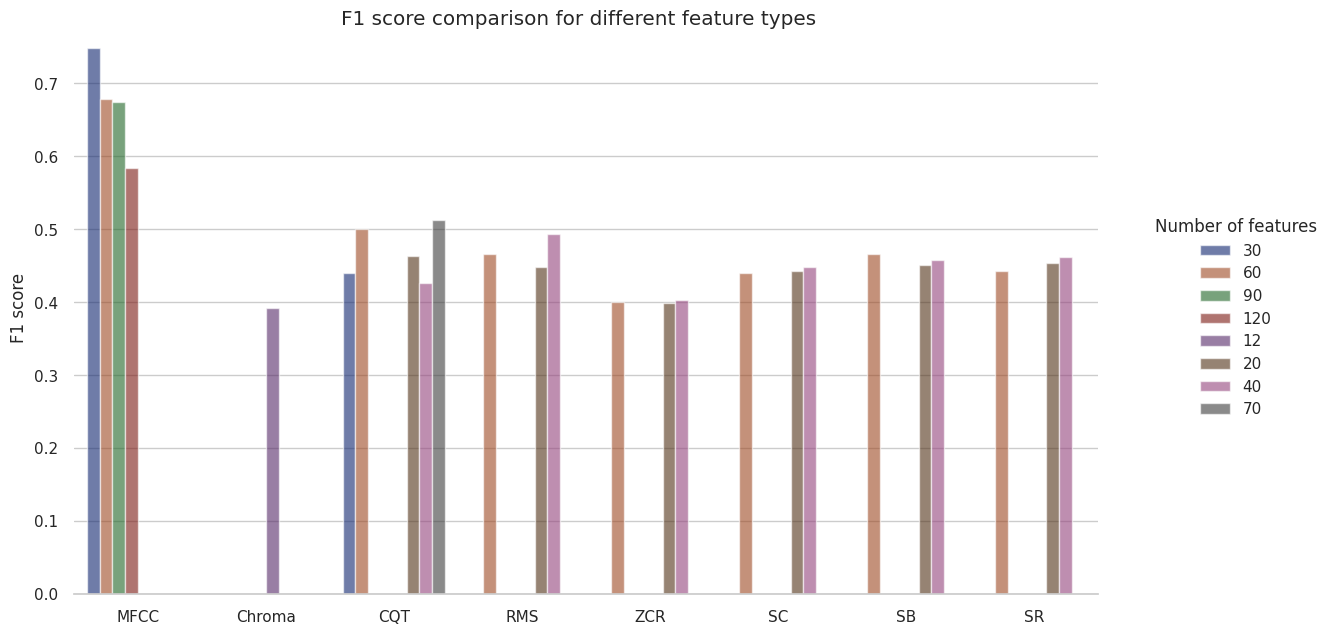
\includegraphics[width=.8\textwidth]{../images/n_feature_per_type.png}
    \caption{F1 score per number of features}
    \label{fig:n_feature_per_type}
\end{figure*}
\noindent
\subsection{Correlation analysis}
The previous analysis resulted in 338 features. Given this large number, it is necessary to perform an analysis to identify and remove features
that are poorly correlated with the target variable as well as those that are highly correlated with each other.
Due to the high number of features, a visual approach, such as a correlation matrix, was not feasible for identifying the features to be removed.
Instead, two filters were applied to select the most relevant features.\\
Since the normality test failed, the Spearman correlation coefficient was used for the analysis.\\
The first filter is based on the correlation between the features and the target variable. Features with a correlation below a certain
threshold with the target variable are removed. The second filter focuses on the correlation among the features themselves.
It counts, for each feature, the number of other features with which it has a correlation above a certain threshold. Features with a
number of correlations above a specified threshold are then removed.\\
The threshold values were chosen empirically. The filters were applied using the combinations of thresholds shown in Table \ref{tab:threshold_values}.

\rowcolors{2}{blue!8}{blue!18}
\begin{table}[h]
    \centering
    \small
    \begin{tabular}{|c|c|c|}
        \hline
        \textbf{Threshold} & \textbf{Values}                 \\
        THRESHOLD 1        & 0 - 0.1 - 0.2 - 0.3 - 0.4 - 0.5 \\
        THRESHOLD 2        & 0.6 - 0.7 - 0.8 - 0.9 - 1       \\
        N° FEATURES        & 5 - 10 - 15 - 20 - 25 - 30 - 40 \\
        \hline
    \end{tabular}
    \caption{threshold values}
    \label{tab:threshold_values}
\end{table}
\noindent
Using the filtered data, Random Forest models were trained to evaluate performance, as Random Forest was found to be the best performing model.
The combination of thresholds that led to the best performance was selected: threshold 1 = 0, threshold 2 = 0.6, and the number of features = 30.\\
From these results, it can be observed that with threshold 1 = 0, the filter on the correlation between the features and the target variable is effectively bypassed.
However, with threshold 2 = 0.6, a stringent filter is applied on the correlation among the features themselves, as all features with a correlation above 0.6
with at least 30 other features are removed. This indicates that it is more detrimental for the model to have features that are highly correlated
with each other than to have features that are poorly correlated with the target variable.\\
Figure \ref{fig:comparison_model_on_all_features_vs_model_on_best} shows the results obtained with the model trained on filtered features
compared to the model trained on all features. As can be seen, the model trained on filtered features performs significantly
better than the one trained on unfiltered features.

\begin{figure}[H]
    \centering
    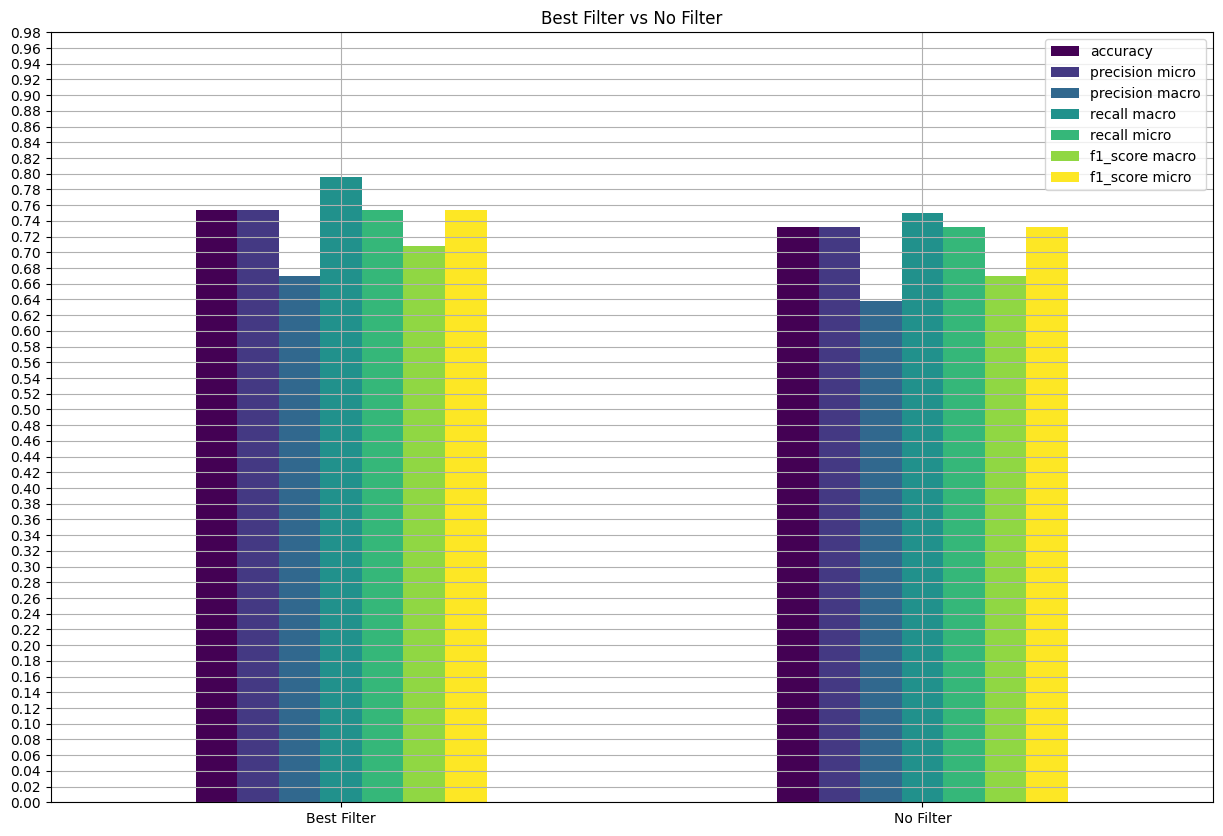
\includegraphics[width=0.8\columnwidth]{../images/model_on_all_features_vs_model_on_best.png}
    \caption{Comparison of different metrics between the model on all features and the model on the filtered ones}
    \label{fig:comparison_model_on_all_features_vs_model_on_best}
\end{figure}
\noindent
From the entire analysis, 41 features remained: 28 MFCC, 12 Chroma, and 1 ZCR.
The correlation matrix of the filtered features is shown in Figure \ref{fig:correlation_matrix}.
This matrix illustrates the pairwise correlation between the selected features, where the color intensity indicates the strength and direction of the correlation.
Dark red cells represent high positive correlations, while dark blue cells indicate high negative correlations.\\
The matrix demonstrates that the remaining features have low correlations with each other, as evidenced by the predominantly light colors away from the diagonal.
This implies that the features are relatively uncorrelated, which helps in preventing multicollinearity issues and enhances the robustness of the model.\\
The high diagonal values indicate that each feature is perfectly correlated with itself, which is expected.
However, the off-diagonal values being close to zero for most feature pairs confirm that the filtering process was effective in selecting
features that do not exhibit high inter-correlations. 

\begin{figure}[H]
    \centering
    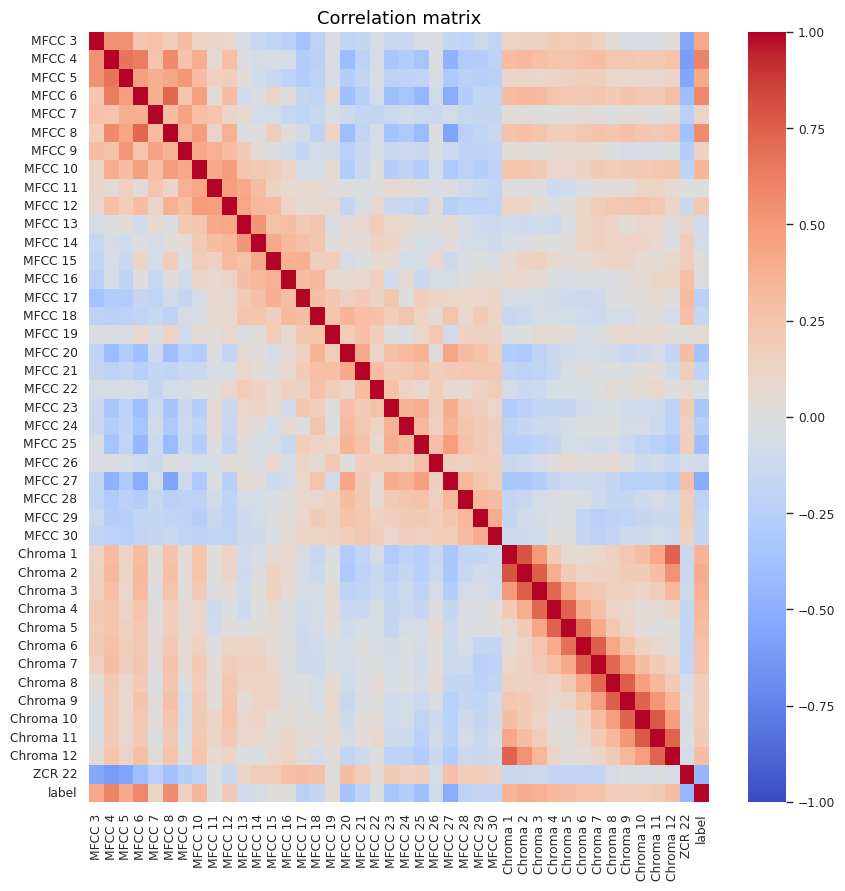
\includegraphics[width=0.8\columnwidth]{../images/correlation_matrix.png}
    \caption{Correlation matrix of the filtered features}
    \label{fig:correlation_matrix}
\end{figure}


% ------------------- Correlation Analysis -------------------
\section{Correlation Analysis}

Given the large number of features (338 in total), it was necessary to identify and remove features that are poorly correlated with
the target variable as well as those that are highly correlated with each other. Due to the high number of features, a visual approach,
such as a correlation matrix, was not feasible. Instead, two filters were applied to select the most
relevant features using the Spearman correlation coefficient, as the normality test failed.

\begin{algorithm}
    \caption{Feature Selection Process}
    \begin{algorithmic}[1]
        \State \textbf{Step 1:} Calculate the Spearman correlation coefficient for each feature with the target variable.
        \State \textbf{Step 2:} Apply the first filter to remove features with a correlation below a certain threshold with the target variable.
        \State \textbf{Step 3:} Calculate the pairwise Spearman correlation coefficients among all features.
        \State \textbf{Step 4:} Apply the second filter to remove features that have a high number of correlations (above a certain threshold)
        with other features.
        \State \textbf{Step 5:} Choose threshold values empirically and apply the filters using various combinations of these thresholds.
        \State \textbf{Step 6:} Train Random Forest models on the filtered data to evaluate performance and select the best combination of thresholds.
    \end{algorithmic}
\end{algorithm}

\subsection{Threshold Selection and Model Evaluation}

Threshold values were chosen empirically and the filters were applied using the combinations shown in Table \ref{tab:threshold_values}.
Using the filtered data, Random Forest models were trained and evaluated, as Random Forest was found to be the best performing model.
The optimal combination of thresholds was found to be: threshold 1 = 0, threshold 2 = 0.6, resulting in 30 features.

\rowcolors{2}{blue!8}{blue!18}
\begin{table}[h]
    \centering
    \small
    \begin{tabular}{|c|c|c|}
        \hline
        \textbf{Threshold} & \textbf{Values}                 \\
        THRESHOLD 1        & 0 - 0.1 - 0.2 - 0.3 - 0.4 - 0.5 \\
        THRESHOLD 2        & 0.6 - 0.7 - 0.8 - 0.9 - 1       \\
        N° FEATURES        & 5 - 10 - 15 - 20 - 25 - 30 - 40 \\
        \hline
    \end{tabular}
    \caption{threshold values}
    \label{tab:threshold_values}
\end{table}
\noindent
With threshold 1 = 0, the filter on the correlation between the features and the target variable was effectively bypassed.
However, with threshold 2 = 0.6, a stringent filter was applied on the correlation among the features themselves,
removing features that had a correlation above 0.6 with at least 30 other features. This indicates that having features
highly correlated with each other is more detrimental to the model than having features poorly correlated with the target variable.\\
Figure \ref{fig:comparison_model_on_all_features_vs_model_on_best} shows the results obtained with the model trained on filtered features
compared to the model trained on all features. As demonstrated, the model trained on filtered features performs significantly better.

\begin{figure}[H]
    \centering
    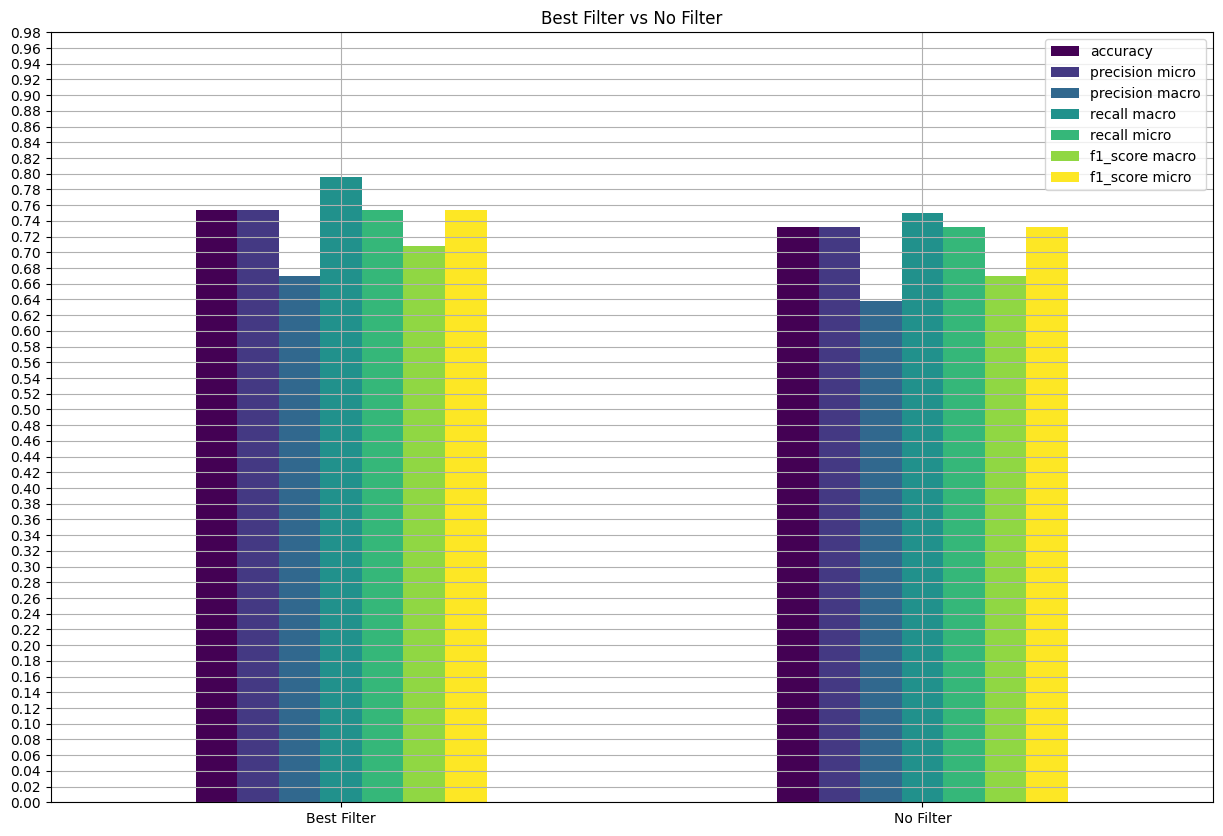
\includegraphics[width=0.8\columnwidth]{../images/model_on_all_features_vs_model_on_best.png}
    \caption{Comparison of different metrics between the model on all features and the model on the filtered ones}
    \label{fig:comparison_model_on_all_features_vs_model_on_best}
\end{figure}

\subsection{Selected Features and Correlation Matrix}

From this analysis, 41 features remained: 28 MFCC, 12 Chroma, and 1 ZCR.
The correlation matrix of the filtered features is shown in Figure \ref{fig:correlation_matrix}.
This matrix illustrates the pairwise correlation between the selected features, with the color intensity
indicating the strength and direction of the correlation. Dark red cells represent high positive correlations,
while dark blue cells indicate high negative correlations.

\begin{figure}[H]
    \centering
    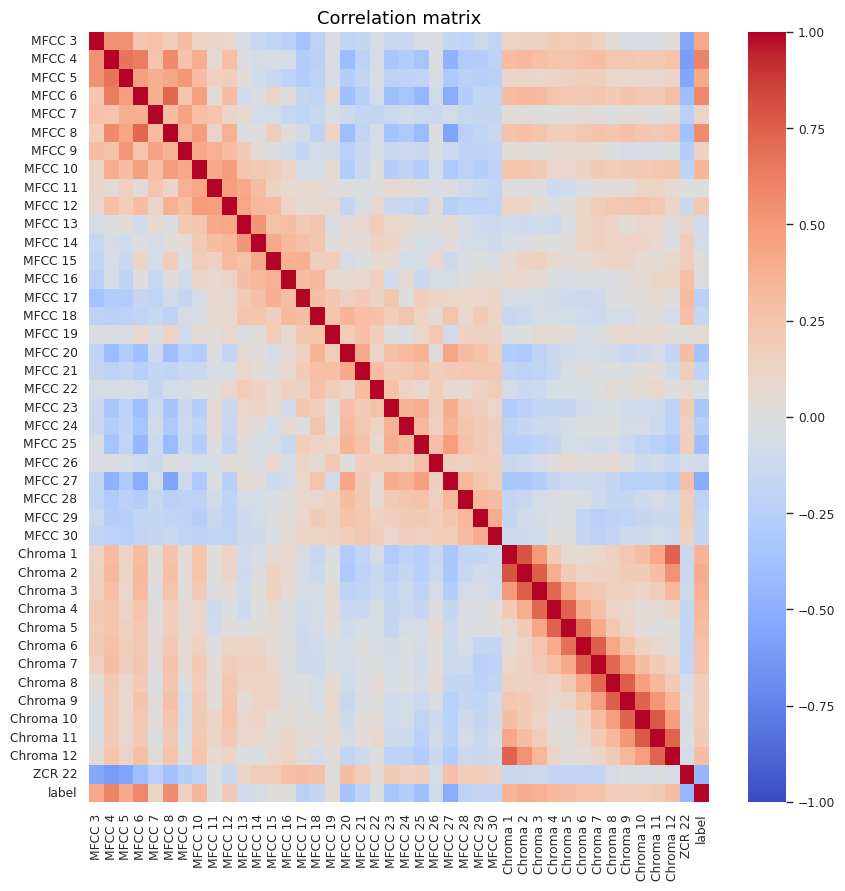
\includegraphics[width=0.8\columnwidth]{../images/correlation_matrix.png}
    \caption{Correlation matrix of the filtered features}
    \label{fig:correlation_matrix}
\end{figure}
\noindent
The matrix demonstrates that the remaining features have low correlations with each other, as evidenced by the predominantly
light colors away from the diagonal. This implies that the features are relatively uncorrelated, preventing multicollinearity
issues and enhancing the robustness of the model. The high diagonal values indicate that each feature is perfectly correlated
with itself, which is expected. However, the off-diagonal values being close to zero for most feature pairs confirm that the filtering
process was effective in selecting features that do not exhibit high inter-correlations.


% % ------------------- Correlation Analysis -------------------
% \section{Correlation Analysis}

Given the large number of features (338 in total), it was necessary to identify and remove features that are poorly correlated with
the target variable as well as those that are highly correlated with each other. Due to the high number of features, a visual approach,
such as a correlation matrix, was not feasible. Instead, two filters were applied to select the most
relevant features using the Spearman correlation coefficient, as the normality test failed.

\begin{algorithm}
    \caption{Feature Selection Process}
    \begin{algorithmic}[1]
        \State \textbf{Step 1:} Calculate the Spearman correlation coefficient for each feature with the target variable.
        \State \textbf{Step 2:} Apply the first filter to remove features with a correlation below a certain threshold with the target variable.
        \State \textbf{Step 3:} Calculate the pairwise Spearman correlation coefficients among all features.
        \State \textbf{Step 4:} Apply the second filter to remove features that have a high number of correlations (above a certain threshold)
        with other features.
        \State \textbf{Step 5:} Choose threshold values empirically and apply the filters using various combinations of these thresholds.
        \State \textbf{Step 6:} Train Random Forest models on the filtered data to evaluate performance and select the best combination of thresholds.
    \end{algorithmic}
\end{algorithm}

\subsection{Threshold Selection and Model Evaluation}

Threshold values were chosen empirically and the filters were applied using the combinations shown in Table \ref{tab:threshold_values}.
Using the filtered data, Random Forest models were trained and evaluated, as Random Forest was found to be the best performing model.
The optimal combination of thresholds was found to be: threshold 1 = 0, threshold 2 = 0.6, resulting in 30 features.

\rowcolors{2}{blue!8}{blue!18}
\begin{table}[h]
    \centering
    \small
    \begin{tabular}{|c|c|c|}
        \hline
        \textbf{Threshold} & \textbf{Values}                 \\
        THRESHOLD 1        & 0 - 0.1 - 0.2 - 0.3 - 0.4 - 0.5 \\
        THRESHOLD 2        & 0.6 - 0.7 - 0.8 - 0.9 - 1       \\
        N° FEATURES        & 5 - 10 - 15 - 20 - 25 - 30 - 40 \\
        \hline
    \end{tabular}
    \caption{threshold values}
    \label{tab:threshold_values}
\end{table}
\noindent
With threshold 1 = 0, the filter on the correlation between the features and the target variable was effectively bypassed.
However, with threshold 2 = 0.6, a stringent filter was applied on the correlation among the features themselves,
removing features that had a correlation above 0.6 with at least 30 other features. This indicates that having features
highly correlated with each other is more detrimental to the model than having features poorly correlated with the target variable.\\
Figure \ref{fig:comparison_model_on_all_features_vs_model_on_best} shows the results obtained with the model trained on filtered features
compared to the model trained on all features. As demonstrated, the model trained on filtered features performs significantly better.

\begin{figure}[H]
    \centering
    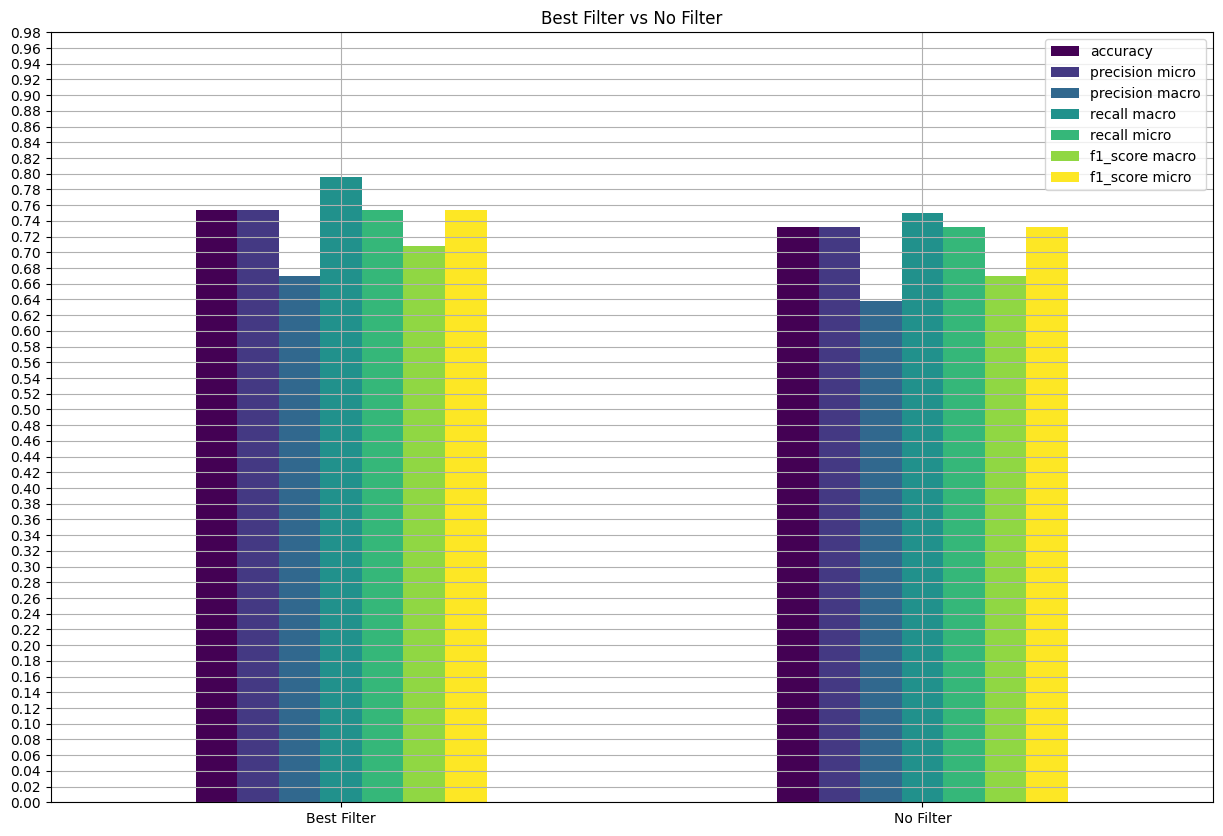
\includegraphics[width=0.8\columnwidth]{../images/model_on_all_features_vs_model_on_best.png}
    \caption{Comparison of different metrics between the model on all features and the model on the filtered ones}
    \label{fig:comparison_model_on_all_features_vs_model_on_best}
\end{figure}

\subsection{Selected Features and Correlation Matrix}

From this analysis, 41 features remained: 28 MFCC, 12 Chroma, and 1 ZCR.
The correlation matrix of the filtered features is shown in Figure \ref{fig:correlation_matrix}.
This matrix illustrates the pairwise correlation between the selected features, with the color intensity
indicating the strength and direction of the correlation. Dark red cells represent high positive correlations,
while dark blue cells indicate high negative correlations.

\begin{figure}[H]
    \centering
    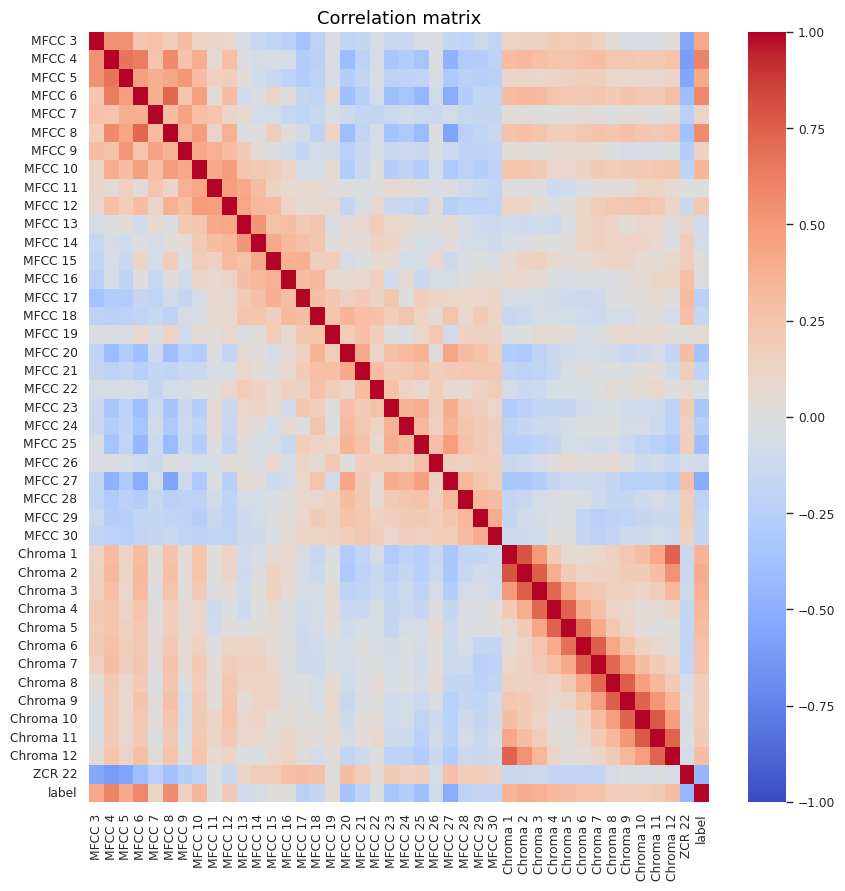
\includegraphics[width=0.8\columnwidth]{../images/correlation_matrix.png}
    \caption{Correlation matrix of the filtered features}
    \label{fig:correlation_matrix}
\end{figure}
\noindent
The matrix demonstrates that the remaining features have low correlations with each other, as evidenced by the predominantly
light colors away from the diagonal. This implies that the features are relatively uncorrelated, preventing multicollinearity
issues and enhancing the robustness of the model. The high diagonal values indicate that each feature is perfectly correlated
with itself, which is expected. However, the off-diagonal values being close to zero for most feature pairs confirm that the filtering
process was effective in selecting features that do not exhibit high inter-correlations.


% ------------------- Model Selection -------------------
\section{Model Selection}
In the large majority of medical problems, 
% \begin{table}[h!]
%     \centering
%     \begin{tabular}{|l|l|}
%         \hline
%         \textbf{Nome}           & \textbf{Architettura}                                 \\ \hline
%         XGBoost                 & -                                                     \\ \hline
%         CatBoost                & -                                                     \\ \hline
%         LightGBM                & -                                                     \\ \hline
%         MLP\_Basic              & (128, 64, 32)                                         \\ \hline
%         MLP\_Ultra              & (512, 256, 128, 64, 32)                               \\ \hline
%         MLP\_Large              & (256, 128, 64, 32)                                    \\ \hline
%         MLP\_Small              & (64, 32)                                              \\ \hline
%         MLP\_Tiny               & (32, 16)                                              \\ \hline
%         MLP\_Reverse            & (32, 64, 128, 256, 512, 256, 128, 64, 32)             \\ \hline
%         MLP\_Bottleneck         & (512, 64, 32)                                         \\ \hline
%         MLP\_Rollercoaster      & (512, 128, 256, 128, 256, 64, 32)                     \\ \hline
%         MLP\_Hourglass          & (512, 256, 128, 64, 32, 64, 128, 256, 512)            \\ \hline
%         MLP\_Pyramid            & (1024, 512, 256, 128, 128, 128, 64, 32)               \\ \hline
%         MLP\_Wide               & (1024, 1024)                                          \\ \hline
%         MLP\_WideUltra          & (1024, 1024, 128, 32)                                 \\ \hline
%         MLP\_Sparse             & (32, 16, 8)                                           \\ \hline
%         MLP\_Dropout            & (128, 64, 32)                                         \\ \hline
%         MLP\_Ensemble1          & \footnotesize{ MLP\_Basic, MLP\_Large, MLP\_Ultra     \\ }\hline
%         MLP\_Ensemble2          & RandomForest, MLP\_Ultra                              \\ \hline
%         MLP\_Ensemble3          & MLP\_Rollercoaster, MLP\_Large                        \\ \hline
%         MLP\_Ensemble4          & MLP\_Rollercoaster, MLP\_Large, MLP\_Ultra            \\ \hline
%         MLP\_Ensemble5          & RandomForest, MLP\_Ultra, MLP\_Rollercoaster          \\ \hline
%         MLP\_Ensemble6          & MLP\_Rollercoaster, MLP\_Large, MLP\_Ultra, MLP\_Wide \\ \hline
%         ALL\_Ensemble           & All models majority vote                              \\ \hline
%         CatBoost\_ALL\_Ensemble & All models CatBoost                                   \\ \hline
%     \end{tabular}
%     \caption{Nomi dei modelli e relative architetture}
%     \label{tab:models}
% \end{table}


\subsection{Models Overview}

\subsubsection{LightGBM}
LightGBM (Light Gradient Boosting Machine) is a gradient boosting framework that builds decision trees in a leaf-wise manner. Unlike level-wise growth used in other boosting algorithms, LightGBM grows trees leaf-wise, leading to better optimization.

The objective function to minimize is:
\begin{equation*}
L = \sum_{i=1}^{n} l(y_i, \hat{y}_i) + \sum_{k} \Omega(f_k)
\end{equation*}
where $l$ is the loss function (e.g., mean squared error for regression), $y_i$ is the true label, $\hat{y}_i$ is the predicted label, and $\Omega$ is the regularization term to avoid overfitting.

\subsubsection{XGBoost}
XGBoost (Extreme Gradient Boosting) enhances the gradient boosting technique by optimizing the loss function using second-order Taylor expansion. The objective function is:
\begin{equation*}
L(\theta) = \sum_{i=1}^{n} l(y_i, \hat{y}_i(t)) + \sum_{k} \Omega(f_k)
\end{equation*}
where $l$ is the loss function, $y_i$ is the true value, $\hat{y}_i(t)$ is the prediction at the $t$-th iteration, and $\Omega(f_k)$ is the regularization term. The regularization term is given by:
\begin{equation*}
\Omega(f) = \gamma T + \frac{1}{2} \lambda \sum_{j=1}^{T} w_j^2
\end{equation*}
where $T$ is the number of leaves, $w_j$ are the leaf weights, and $\gamma$ and $\lambda$ are regularization parameters.

\subsubsection{CatBoost}
CatBoost (Categorical Boosting) is designed to handle categorical features natively. It uses ordered boosting to avoid overfitting and provides efficient handling of categorical data without extensive preprocessing. The model learns using the following objective function:
\begin{equation*}
L = \sum_{i=1}^{n} l(y_i, \hat{y}_i) + \lambda \sum_{j=1}^{m} ||w_j||^2
\end{equation*}
where $l$ is the loss function, $y_i$ is the true label, $\hat{y}_i$ is the predicted label, $\lambda$ is the regularization parameter, and $w_j$ are the model weights.

\subsubsection{Random Forest}
Random Forest is an ensemble method that builds multiple decision trees using bootstrap samples and random feature subsets. The final prediction is made by averaging the predictions (regression) or majority voting (classification). The prediction for a regression problem is:
\begin{equation*}
\hat{y} = \frac{1}{T} \sum_{t=1}^{T} h_t(x)
\end{equation*}
where $T$ is the number of trees, $h_t$ is the prediction of the $t$-th tree, and $x$ is the input feature vector.

\subsubsection{MLP (Multilayer Perceptron)}
MLP (Multilayer Perceptron) is a type of feedforward neural network with one or more hidden layers. Each neuron computes a weighted sum of inputs, applies an activation function, and passes the result to the next layer. The output of a neuron in layer $l$ is:
\begin{equation*}
a_i^{(l)} = f \left( \sum_{j=1}^{n^{(l-1)}} w_{ij}^{(l)} a_j^{(l-1)} + b_i^{(l)} \right)
\end{equation*}
where $a_i^{(l)}$ is the activation of the $i$-th neuron in layer $l$, $w_{ij}^{(l)}$ is the weight between neuron $j$ in layer $l-1$ and neuron $i$ in layer $l$, $b_i^{(l)}$ is the bias term, and $f$ is the activation function (e.g., ReLU, sigmoid).

\end{document}



\subsection{Multiclass Model}
\subusubsection{Results}
\subusubsection{Risk Score}

\subsection{Normal VS Rest Model}
\subsubsection{FPR Oriented Model}
\subsubsection{Results}

\subsection{Diseases Only Model}
\subsubsection{Results}

% ------------------- Best Model Analysis -------------------
\section{Analysis of the Best Model}

% ---------------------- Conclusion -----------------------------

\section{Conclusion}
\section{Future Works}
% - our approach in feature selection and parameters search is not optimal 
% - list the possible issues (e.g. we are training model on diverse features with the optimal parameters for other features)
% - exploit the knowledge of symptoms communities and their most pointed diseases, using it at prior probability for the model classification

\clearpage
\section{Appendix}

% Figure on the best prevention model


% color the image in black
\begin{figure}[H]
    \centering
    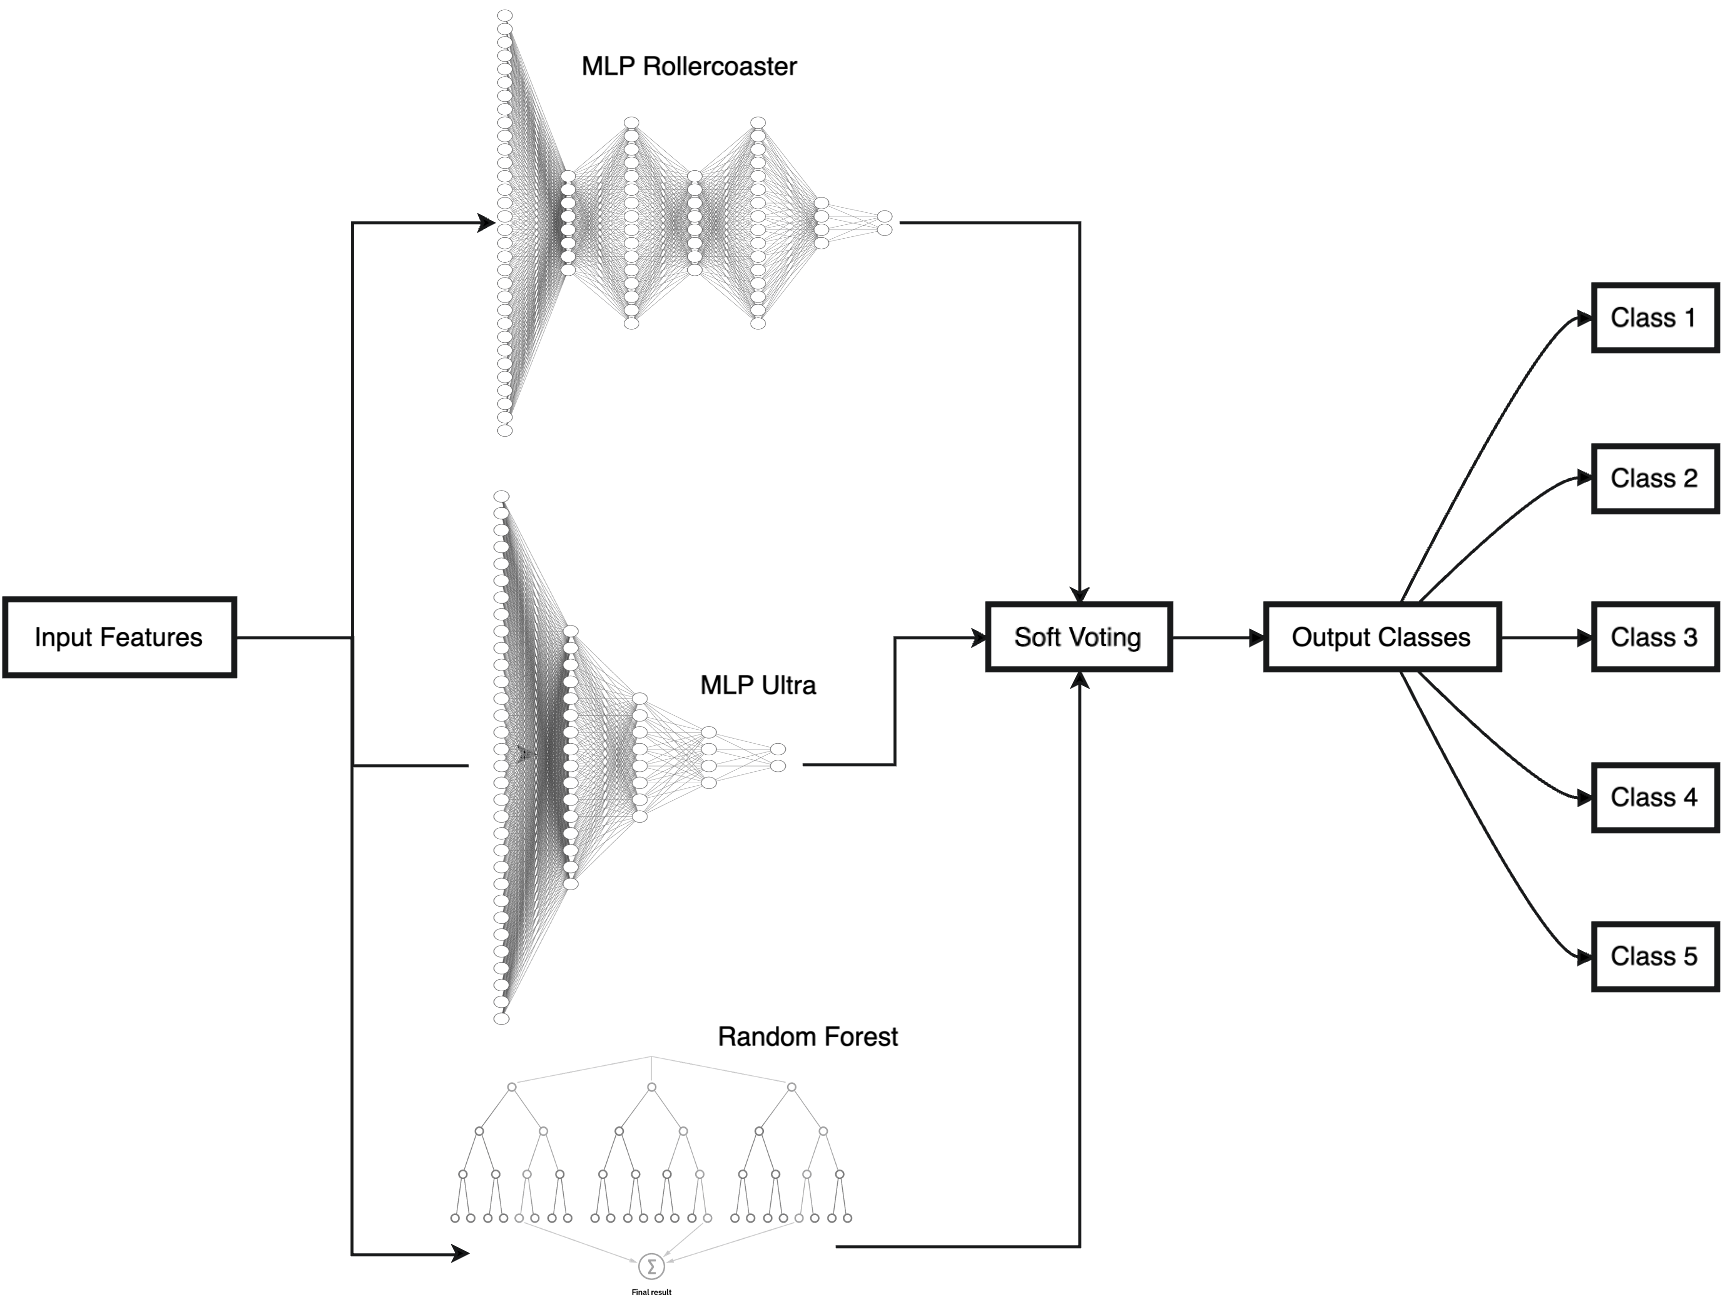
\includegraphics[width=1\columnwidth]{./images/MLP_Ensemble5.png}
    \caption{MLP Ensemble5 Architecture}
    \label{fig:MLP_Ensemble5}
\end{figure}

\clearpage
\printbibliography

\end{document}